\begin{remark}
  Si $M, M'$ son $A$-módulos, $g:M\to M'$ es suprayectiva, y $N\subset \ker g$, entonces el siguiente diagrama conmuta
  \tikzset{every picture/.style={line width=0.75pt}} %set default line width to 0.75pt

  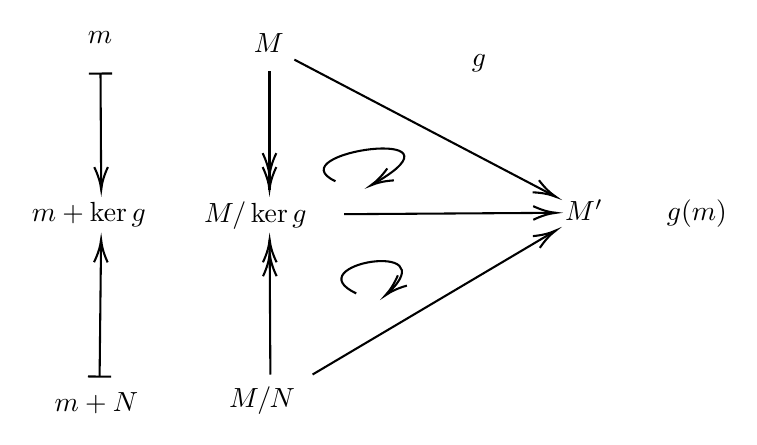
\begin{tikzpicture}[x=0.75pt,y=0.75pt,yscale=-1,xscale=1]
  %uncomment if require: \path (0,300); %set diagram left start at 0, and has height of 300

  %Curve Lines [id:da06639929221173313]
  \draw    (291.8,208.9) .. controls (262.25,195.11) and (335.54,182.29) .. (307.17,208.67) ;
  \draw [shift={(305.8,209.9)}, rotate = 318.81] [color={rgb, 255:red, 0; green, 0; blue, 0 }  ][line width=0.75]    (10.93,-3.29) .. controls (6.95,-1.4) and (3.31,-0.3) .. (0,0) .. controls (3.31,0.3) and (6.95,1.4) .. (10.93,3.29)   ;
  %Curve Lines [id:da2113069658179978]
  \draw    (281.8,154.9) .. controls (252.1,141.04) and (350.79,127.18) .. (300.37,156.01) ;
  \draw [shift={(298.8,156.9)}, rotate = 330.95] [color={rgb, 255:red, 0; green, 0; blue, 0 }  ][line width=0.75]    (10.93,-3.29) .. controls (6.95,-1.4) and (3.31,-0.3) .. (0,0) .. controls (3.31,0.3) and (6.95,1.4) .. (10.93,3.29)   ;

  % Text Node
  \draw (241,82.4) node [anchor=north west][inner sep=0.75pt]    {$M$};
  % Text Node
  \draw (391,162.4) node [anchor=north west][inner sep=0.75pt]    {$M'$};
  % Text Node
  \draw (346,92.4) node [anchor=north west][inner sep=0.75pt]    {$g$};
  % Text Node
  \draw (217,163.4) node [anchor=north west][inner sep=0.75pt]    {$M/\ker g$};
  % Text Node
  \draw (229,252.4) node [anchor=north west][inner sep=0.75pt]    {$M/N$};
  % Text Node
  \draw (145,255.4) node [anchor=north west][inner sep=0.75pt]    {$m+N$};
  % Text Node
  \draw (134,163.4) node [anchor=north west][inner sep=0.75pt]    {$m+\ker g$};
  % Text Node
  \draw (161,81.4) node [anchor=north west][inner sep=0.75pt]    {$m$};
  % Text Node
  \draw (440,162.4) node [anchor=north west][inner sep=0.75pt]    {$g( m)$};
  % Connection
  \draw    (262,96.3) -- (386.23,161.46) ;
  \draw [shift={(388,162.39)}, rotate = 207.68] [color={rgb, 255:red, 0; green, 0; blue, 0 }  ][line width=0.75]    (10.93,-3.29) .. controls (6.95,-1.4) and (3.31,-0.3) .. (0,0) .. controls (3.31,0.3) and (6.95,1.4) .. (10.93,3.29)   ;
  % Connection
  \draw    (250,102) -- (250,159) ;
  \draw [shift={(250,159)}, rotate = 270] [color={rgb, 255:red, 0; green, 0; blue, 0 }  ][line width=0.75]    (17.64,-3.29) .. controls (13.66,-1.4) and (10.02,-0.3) .. (6.71,0) .. controls (10.02,0.3) and (13.66,1.4) .. (17.64,3.29)(10.93,-3.29) .. controls (6.95,-1.4) and (3.31,-0.3) .. (0,0) .. controls (3.31,0.3) and (6.95,1.4) .. (10.93,3.29)   ;
  % Connection
  \draw    (250.43,248) -- (250.07,183) ;
  \draw [shift={(250.07,183)}, rotate = 449.68] [color={rgb, 255:red, 0; green, 0; blue, 0 }  ][line width=0.75]    (17.64,-3.29) .. controls (13.66,-1.4) and (10.02,-0.3) .. (6.71,0) .. controls (10.02,0.3) and (13.66,1.4) .. (17.64,3.29)(10.93,-3.29) .. controls (6.95,-1.4) and (3.31,-0.3) .. (0,0) .. controls (3.31,0.3) and (6.95,1.4) .. (10.93,3.29)   ;
  % Connection
  \draw    (270.77,248) -- (386.28,179.6) ;
  \draw [shift={(388,178.59)}, rotate = 509.37] [color={rgb, 255:red, 0; green, 0; blue, 0 }  ][line width=0.75]    (10.93,-3.29) .. controls (6.95,-1.4) and (3.31,-0.3) .. (0,0) .. controls (3.31,0.3) and (6.95,1.4) .. (10.93,3.29)   ;
  % Connection
  \draw    (286,170.76) -- (386,170.11) ;
  \draw [shift={(388,170.1)}, rotate = 539.62] [color={rgb, 255:red, 0; green, 0; blue, 0 }  ][line width=0.75]    (10.93,-3.29) .. controls (6.95,-1.4) and (3.31,-0.3) .. (0,0) .. controls (3.31,0.3) and (6.95,1.4) .. (10.93,3.29)   ;
  % Connection
  \draw    (168.15,249) -- (168.85,185) ;
  \draw [shift={(168.87,183)}, rotate = 450.62] [color={rgb, 255:red, 0; green, 0; blue, 0 }  ][line width=0.75]    (10.93,-3.29) .. controls (6.95,-1.4) and (3.31,-0.3) .. (0,0) .. controls (3.31,0.3) and (6.95,1.4) .. (10.93,3.29)   ;
  \draw [shift={(168.15,249)}, rotate = 450.62] [color={rgb, 255:red, 0; green, 0; blue, 0 }  ][line width=0.75]    (0,5.59) -- (0,-5.59)   ;
  % Connection
  \draw    (168.59,103) -- (168.91,157) ;
  \draw [shift={(168.93,159)}, rotate = 269.65] [color={rgb, 255:red, 0; green, 0; blue, 0 }  ][line width=0.75]    (10.93,-3.29) .. controls (6.95,-1.4) and (3.31,-0.3) .. (0,0) .. controls (3.31,0.3) and (6.95,1.4) .. (10.93,3.29)   ;
  \draw [shift={(168.59,103)}, rotate = 269.65] [color={rgb, 255:red, 0; green, 0; blue, 0 }  ][line width=0.75]    (0,5.59) -- (0,-5.59)   ;

  \end{tikzpicture}
\end{remark}
